% Sensing depth of a periodic electrode array: derivation of the lambda/2pi rule.
% Build (MiKTeX, installer disabled so it never prompts):
%   pdflatex --disable-installer -interaction=nonstopmode MSV4_SENSING_DEPTH_DERIVATION_2026-09-30.tex  (x2)
% Numbers in Section 5: MSV4/scripts/msv4_sensing_depth_figure.py and the sources cited there.
\documentclass[11pt,letterpaper]{article}
% US letter, 1 in margins, set directly (geometry.sty is not installed here)
\pdfpagewidth=8.5in \pdfpageheight=11in
\setlength{\textwidth}{6.5in}\setlength{\oddsidemargin}{0in}\setlength{\evensidemargin}{0in}
\setlength{\headheight}{14pt}\setlength{\headsep}{0.1in}\setlength{\topmargin}{-0.3in}
\setlength{\textheight}{9in}\setlength{\footskip}{0.45in}
\usepackage[T1]{fontenc}
\usepackage{lmodern}
\usepackage{microtype}
\usepackage{amsmath,amssymb,mathtools}
\usepackage{booktabs}
\usepackage{xcolor}
\usepackage{tikz}
\usepackage{tcolorbox}
\usepackage{enumitem}
\usepackage{fancyhdr}
\usepackage{titlesec}
\usepackage{caption}

\definecolor{ink}{HTML}{1B1B1B}
\definecolor{inkgray}{HTML}{5A5A5A}
\definecolor{soil}{HTML}{F5EFE4}
\definecolor{board}{HTML}{E2E5E9}
\definecolor{hot}{HTML}{1F4E8C}
\definecolor{gnd}{HTML}{9AA3AD}

\titleformat{\section}{\normalfont\large\bfseries}{\thesection}{0.8em}{}
\titlespacing*{\section}{0pt}{1.5em}{0.6em}
\captionsetup{font=small,labelfont=bf,margin=12pt}
\setlist{itemsep=2pt,topsep=4pt}

\pagestyle{fancy}
\fancyhf{}
\renewcommand{\headrulewidth}{0pt}
\fancyfoot[L]{\footnotesize\color{inkgray}Project Treebeard \textperiodcentered{} MSV4 electrode notes}
\fancyfoot[R]{\footnotesize\color{inkgray}\thepage}

\newcommand{\e}{\mathrm{e}}
\newcommand{\dd}{\,\mathrm{d}}
\newcommand{\eff}{\mathrm{eff}}

\begin{document}

\begin{center}
{\LARGE\bfseries Sensing depth of a periodic electrode array}\\[6pt]
{\large Why the depth scale is $\lambda/2\pi$, and how much of the signal comes from within depth $d$}\\[8pt]
{\small\color{inkgray}Project Treebeard \textperiodcentered{} MSV4 electrode notes \textperiodcentered{} 30 September 2026}
\end{center}

\vspace{4pt}
\begin{tcolorbox}[colback=gray!4,colframe=gray!45,boxrule=0.5pt,arc=2pt,left=10pt,right=10pt,top=6pt,bottom=6pt]
\textbf{Results.} For electrodes that alternate driven and ground with centre-to-centre spacing $s$, the
pattern repeats every $\lambda = 2s$, and
\begin{align*}
  \text{1/e depth of the field:}\qquad & \delta = \frac{\lambda}{2\pi}, \\[2pt]
  \text{share from within } d\text{, weak contrast:}\qquad & S(d) = 1-\e^{-4\pi d/\lambda}, \\[2pt]
  \text{share from within } d\text{, soil } \varepsilon_1 \text{ over air } \varepsilon_2\text{:}\qquad &
  S(d) = \frac{(1+\rho)\tanh(2\pi d/\lambda)}{1+\rho\tanh(2\pi d/\lambda)}, \quad \rho = \frac{\varepsilon_2}{\varepsilon_1}.
\end{align*}
The pattern enters only through $\lambda$. For a periodic pattern each result is an upper bound on how deep
the sensor looks (the third under a fixed surface potential, Section~4); higher harmonics only make the
response shallower.
\end{tcolorbox}

\section{Setup}

\begin{figure}[h]
\centering
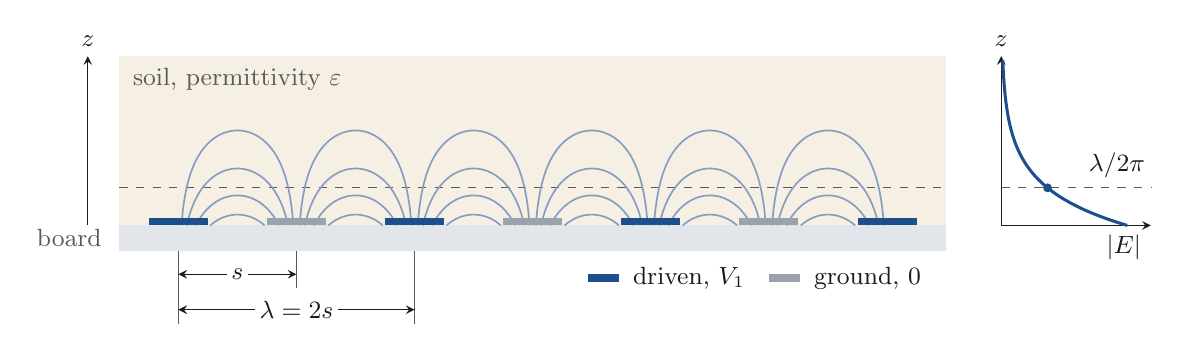
\begin{tikzpicture}[x=1cm,y=1cm,>=stealth]
  \def\L{3}
  % soil and board
  \fill[soil] (-0.75,0) rectangle (9.75,2.15);
  \fill[board] (-0.75,-0.32) rectangle (9.75,0);
  \node[anchor=north west,font=\small,text=inkgray] at (-0.7,2.12) {soil, permittivity $\varepsilon$};
  \node[anchor=east,font=\small,text=inkgray] at (-0.85,-0.16) {board};
  % 1/e depth of the fundamental
  \draw[inkgray,dashed,thin] (-0.75,{\L/(2*pi)}) -- (9.75,{\L/(2*pi)});
  % exact field lines of the fundamental: sin(kx) e^{-kz} = c
  \foreach \m in {0,...,5}{
    \foreach \c in {0.08,0.22,0.45,0.75}{
      \pgfmathsetmacro{\xa}{asin(\c)/360*\L}
      \pgfmathsetmacro{\xs}{\m*\L/2+\xa}
      \pgfmathsetmacro{\xe}{(\m+1)*\L/2-\xa}
      \draw[hot!55,line width=0.6pt] plot[domain=\xs:\xe,samples=70,smooth]
        (\x,{max(0,\L/(2*pi)*ln(max(1e-6,abs(sin(360*\x/\L)))/\c))});
    }
  }
  % electrodes
  \foreach \i in {0,2,4,6}{\fill[hot] ({\i*\L/2-0.375},0) rectangle ({\i*\L/2+0.375},0.09);}
  \foreach \i in {1,3,5}{\fill[gnd] ({\i*\L/2-0.375},0) rectangle ({\i*\L/2+0.375},0.09);}
  % dimensions
  \draw[inkgray,thin] (0,-0.32) -- (0,-1.25);
  \draw[inkgray,thin] (1.5,-0.32) -- (1.5,-0.8);
  \draw[inkgray,thin] (3,-0.32) -- (3,-1.25);
  \draw[<->,ink] (0,-0.62) -- node[fill=white,inner sep=1.5pt,font=\small]{$s$} (1.5,-0.62);
  \draw[<->,ink] (0,-1.07) -- node[fill=white,inner sep=1.5pt,font=\small]{$\lambda = 2s$} (3,-1.07);
  % electrode key
  \fill[hot] (5.2,-0.72) rectangle (5.6,-0.62);
  \node[anchor=west,font=\small,text=ink] at (5.65,-0.67) {driven, $V_1$};
  \fill[gnd] (7.5,-0.72) rectangle (7.9,-0.62);
  \node[anchor=west,font=\small,text=ink] at (7.95,-0.67) {ground, $0$};
  % z axis
  \draw[->,ink] (-1.15,0) -- (-1.15,2.15) node[above,font=\small]{$z$};
  % right panel: field magnitude of the fundamental
  \draw[->,ink] (10.45,0) -- (10.45,2.15) node[above,font=\small]{$z$};
  \draw[->,ink] (10.45,0) -- (12.35,0) node[below left,font=\small]{$|E|$};
  \draw[hot,line width=1.1pt] plot[domain=0:2.1,samples=60,smooth] ({10.45+1.6*exp(-2*pi*\x/\L)},\x);
  \draw[inkgray,dashed,thin] (10.45,{\L/(2*pi)}) -- (12.35,{\L/(2*pi)});
  \node[anchor=south east,font=\small,text=ink] at (12.4,{\L/(2*pi)}) {$\lambda/2\pi$};
  \fill[hot] ({10.45+1.6*exp(-1)},{\L/(2*pi)}) circle (1.6pt);
\end{tikzpicture}
\caption{Cross-section across the blade (to scale in units of $\lambda$). Electrodes alternate driven and
ground at centre spacing $s$, so the surface pattern repeats every $\lambda = 2s$. The curves are exact
field lines of the fundamental harmonic (Section~2). Right: its field magnitude, which has fallen to
$1/\e$ at the dashed line $z = \lambda/2\pi$.}
\end{figure}

Coordinates: $x$ runs across the blade, $y$ along it, and $z$ into the soil from the electrode plane
$z = 0$.

\begin{enumerate}[label=(A\arabic*),leftmargin=3.2em]
  \item \textbf{Two-dimensional, quasi-static.} The blade is long compared with $\lambda$, so nothing
        varies with $y$. At MHz frequencies the free-space wavelength (hundreds of metres) dwarfs the
        electrodes, so the field obeys electrostatics.
  \item \textbf{Periodic surface potential.} On $z = 0$ the potential $f(x)$ satisfies
        $f(x+\lambda) = f(x)$. Its values across the gaps between electrodes are never needed, only its
        period.
  \item \textbf{Uniform soil.} The half-space $z > 0$ is linear, isotropic and homogeneous, with no free
        charge. For conductive soil at angular frequency $\omega$, replace $\varepsilon$ by
        $\varepsilon - j\sigma/\omega$; a homogeneous medium still obeys Laplace's equation, so
        Section~2 is unchanged.
  \item \textbf{Bounded far field.} $V$ stays bounded as $z \to \infty$.
\end{enumerate}

\section{The potential in the soil: the $\lambda/2\pi$ rule}

With no free charge in a uniform medium, Gauss's law reduces to Laplace's equation:
\begin{equation}
  \frac{\partial^2 V}{\partial x^2} + \frac{\partial^2 V}{\partial z^2} = 0, \qquad z > 0.
  \label{eq:laplace}
\end{equation}
By (A2) the surface potential has a Fourier series,
\begin{equation}
  f(x) = a_0 + \sum_{n=1}^{\infty} \bigl( a_n \cos k_n x + b_n \sin k_n x \bigr),
  \qquad k_n = \frac{2\pi n}{\lambda}.
  \label{eq:fourier}
\end{equation}

\paragraph{Separation of variables.} Try $V = X(x)\,Z(z)$. Substituting into \eqref{eq:laplace} and
dividing by $XZ$ gives $X''/X = -Z''/Z$. The left side depends only on $x$ and the right only on $z$, so
both equal a constant, $-k^2$:
\begin{equation}
  X'' + k^2 X = 0, \qquad Z'' - k^2 Z = 0.
  \label{eq:separated}
\end{equation}
Periodicity (A2) admits only $k = k_n$, with $X = \cos k_n x$ or $\sin k_n x$. Then
$Z = A\,\e^{-k_n z} + B\,\e^{+k_n z}$, and for $n \ge 1$ the growing term violates (A4), so $B = 0$. For
$n = 0$, $Z = A + Bz$, and (A4) again forces $B = 0$. Superposing, and matching \eqref{eq:fourier} at
$z = 0$:
\begin{equation}
  \boxed{\;V(x,z) = a_0 + \sum_{n=1}^{\infty} \bigl( a_n \cos k_n x + b_n \sin k_n x \bigr)\,\e^{-2\pi n z/\lambda}\;}
  \label{eq:solution}
\end{equation}
This satisfies \eqref{eq:laplace} term by term, equals $f$ on $z = 0$, and is bounded. It is the only
such solution.\footnote{The difference of two bounded solutions is harmonic and vanishes on $z = 0$. Its
odd reflection into $z < 0$ is bounded and harmonic on the whole plane, hence constant by Liouville's
theorem, hence zero.} The field $\mathbf{E} = -\nabla V$ is
\begin{equation}
  E_x = \sum_{n=1}^{\infty} k_n \bigl( a_n \sin k_n x - b_n \cos k_n x \bigr)\,\e^{-k_n z}, \qquad
  E_z = \sum_{n=1}^{\infty} k_n \bigl( a_n \cos k_n x + b_n \sin k_n x \bigr)\,\e^{-k_n z}.
  \label{eq:field}
\end{equation}
The constant $a_0$ carries no field. Harmonic $n$ decays at rate $k_n = 2\pi n/\lambda$, so relative to
the fundamental it is suppressed by $\e^{-(n-1)2\pi z/\lambda}$, and a short distance from the surface
only $n = 1$ remains. Its $1/\e$ depth is
\begin{equation}
  \boxed{\;\delta = \frac{1}{k_1} = \frac{\lambda}{2\pi}\;}
  \label{eq:delta}
\end{equation}
Only $\lambda$ appears. Finger count, finger length and board area do not, and by (A3) neither do
frequency or conductivity. Electrode widths enter only through the coefficients $a_n, b_n$: they set how
strong the field is, not how fast it decays.

\section{Where the signal comes from: energy, not field}

Capacitance measures stored energy, $W = \tfrac12 C V_1^2$. To first order, raising the permittivity by
$\delta\varepsilon$ over a region $\Omega$ of the cross-section changes the capacitance per unit length by
\begin{equation}
  \delta C = \frac{1}{V_1^2} \int_\Omega \delta\varepsilon\, |\mathbf{E}|^2 \dd A,
  \label{eq:perturb}
\end{equation}
where the field redistribution contributes only at second order. The share of the response from soil
within depth $d$ is therefore the share of $|\mathbf{E}|^2$ stored there, not the share of
$|\mathbf{E}|$.

For a single harmonic, \eqref{eq:field} gives
$E_x^2 + E_z^2 = k_n^2 c_n^2\, \e^{-2k_n z}$ at every $x$, with $c_n^2 = a_n^2 + b_n^2$, because
$(a\sin\theta - b\cos\theta)^2 + (a\cos\theta + b\sin\theta)^2 = a^2 + b^2$. Cross terms between different
harmonics average to zero over one period, so
\begin{equation}
  \bigl\langle |\mathbf{E}|^2 \bigr\rangle_x (z) = \sum_{n=1}^{\infty} k_n^2 c_n^2\, \e^{-2k_n z}.
  \label{eq:energy}
\end{equation}
The exponent is $2k_n$: energy decays twice as fast as the field. Integrating from $0$ to $d$ and
normalising,\footnote{The sums converge because the field energy per period is finite; the
$r^{-1/2}$ field singularity at an electrode edge is square-integrable.}
\begin{equation}
  S(d) = \frac{\int_0^d \langle |\mathbf{E}|^2\rangle_x \dd z}{\int_0^\infty \langle |\mathbf{E}|^2\rangle_x \dd z}
       = \frac{\sum_n k_n c_n^2 \bigl( 1 - \e^{-2k_n d} \bigr)}{\sum_n k_n c_n^2}.
  \label{eq:share}
\end{equation}
For the fundamental alone,
\begin{equation}
  \boxed{\;S_1(d) = 1 - \e^{-4\pi d/\lambda}\;}
  \label{eq:share1}
\end{equation}
whose $1/\e$ depth is $\lambda/4\pi$; half the signal comes from within $d_{1/2} = (\ln 2/4\pi)\,\lambda
\approx 0.055\,\lambda$. Because $k_n \ge k_1$, every bracket in \eqref{eq:share} is at least
$1 - \e^{-2k_1 d}$, so
\begin{equation}
  S(d) \;\ge\; 1 - \e^{-4\pi d/\lambda}.
  \label{eq:bound}
\end{equation}
Harmonics only make the response shallower; the fundamental sets the deepest reach.

\medskip\noindent
\emph{Note.} The rule $1 - \e^{-2\pi d/\lambda}$ in the 2026-09-15 architecture note uses the decay
rate of the field in place of that of the energy. It matches neither limit derived here, though its
initial slope, $2\pi d/\lambda$, equals that of the strong-contrast limit in Section~4.

\section{Strong contrast: soil over air}

Equation \eqref{eq:perturb} is first order in $\delta\varepsilon$. The field solve instead fills
$0 < z < d$ with soil ($\varepsilon_1$) and $z > d$ with air ($\varepsilon_2$), and reports
\[
  S(d) = \frac{C(d) - C(0)}{C(\infty) - C(0)}
\]
at $\varepsilon_1/\varepsilon_2 = 20$, which is far from a small perturbation. For one harmonic it can be
solved exactly. Hold the surface potential at $V_0\cos kx$.\footnote{For a real multi-harmonic pattern
this assumes the potential across the gaps does not redistribute as the soil changes. It is exact for a
single harmonic.} The solutions of \eqref{eq:laplace} are
\begin{equation}
  V = \bigl( A\,\e^{-kz} + B\,\e^{kz} \bigr)\cos kx \quad (0 < z < d), \qquad
  V = C\,\e^{-kz}\cos kx \quad (z > d).
  \label{eq:layer}
\end{equation}
At $z = d$ the potential and the normal displacement $\varepsilon E_z$ are continuous:
\begin{equation}
  A\,\e^{-kd} + B\,\e^{kd} = C\,\e^{-kd}, \qquad
  \varepsilon_1 \bigl( A\,\e^{-kd} - B\,\e^{kd} \bigr) = \varepsilon_2\, C\,\e^{-kd}.
  \label{eq:bc}
\end{equation}
Eliminating $C$,
\begin{equation}
  B = r\,\e^{-2kd} A, \qquad r = \frac{\varepsilon_1 - \varepsilon_2}{\varepsilon_1 + \varepsilon_2}.
  \label{eq:reflect}
\end{equation}
The charge the soil draws from the electrode plane is $D_z(0^+) = \varepsilon_1 k (A - B)\cos kx$, with
$A + B = V_0$. Writing it as $\varepsilon_\eff\, k V_0 \cos kx$ defines the permittivity the electrodes
effectively see:
\begin{equation}
  \varepsilon_\eff(d)
  = \varepsilon_1\, \frac{1 - r\,\e^{-2kd}}{1 + r\,\e^{-2kd}}
  = \varepsilon_1\, \frac{\varepsilon_2 + \varepsilon_1 \tanh kd}{\varepsilon_1 + \varepsilon_2 \tanh kd}.
  \label{eq:eeff}
\end{equation}
The soil-side capacitance is proportional to $\varepsilon_\eff$, with $\varepsilon_\eff(0) =
\varepsilon_2$ and $\varepsilon_\eff(\infty) = \varepsilon_1$. With $\rho = \varepsilon_2/\varepsilon_1$
and $t = \tanh kd$,
\begin{equation}
  \boxed{\;S(d) = \frac{\varepsilon_\eff - \varepsilon_2}{\varepsilon_1 - \varepsilon_2}
  = \frac{(1+\rho)\,t}{1 + \rho\, t}, \qquad t = \tanh\frac{2\pi d}{\lambda}\;}
  \label{eq:sfinite}
\end{equation}
\textbf{Limits.} As $\rho \to 1$ (weak contrast), $S = 2t/(1+t) = 1 - \e^{-2kd}$, recovering
\eqref{eq:share1}. As $\rho \to 0$ (strong contrast), $S = \tanh kd$. Since $\partial S/\partial\rho = t(1-t)/(1+\rho t)^2 \ge 0$,
strong contrast gives the deepest response, and
\begin{equation}
  \tanh\frac{2\pi d}{\lambda} \;\le\; S(d) \;\le\; 1 - \e^{-4\pi d/\lambda}.
  \label{eq:sandwich}
\end{equation}
\textbf{Median depth.} Setting $S = \tfrac12$ gives $t = 1/(2+\rho)$, so
\begin{equation}
  d_{1/2} = \frac{\lambda}{2\pi}\,\operatorname{artanh}\frac{1}{2+\rho}.
  \label{eq:median}
\end{equation}
For soil at $\varepsilon_r = 20$ over air, $\rho = 0.05$ and $d_{1/2} = 0.0849\,\lambda$. Since $S$
increases with $kd$, higher harmonics again only make the response shallower, so \eqref{eq:median} with
$k = k_1$ bounds the depth of a periodic pattern from above.

\section{Comparison with the field solve}

\begin{table}[h]
\centering
\small
\setlength{\tabcolsep}{5pt}
\renewcommand{\arraystretch}{1.25}
\begin{tabular}{@{}lcccccc@{}}
\toprule
 & & $\lambda/2\pi$ & field rate & energy, weak & soil over air & 2D field \\
Electrode & $\lambda$ & (1/e field) & $\tfrac{\ln 2}{2\pi}\lambda$ & contrast \eqref{eq:share1} &
$\rho = \tfrac{1}{20}$ \eqref{eq:median} & solve \\
\midrule
MSV3 IDE (0.5 / 1.0)                & 3.0  & 0.48 & 0.33 & 0.17 & 0.25 & $\approx$0.23 \\
v1.2 (G3.5 / 2 / H9.5 / 2 / G3.5)   & 17.0 & 2.71 & 1.88 & 0.94 & 1.44 & 1.39 \\
MSV4 as drawn (A|B + guard) & 18.9 & 3.01 & 2.09 & 1.04 & 1.60 & 1.01 \\
\bottomrule
\end{tabular}
\caption{Median depth $d_{1/2}$ in mm ($\lambda/2\pi$ is the 1/e field depth, for reference). Solve:
lossless soil $\varepsilon_r = 20$ over air, 1.6\,mm FR4, 20\,$\mu$m mask; medians interpolated linearly
between solved depths. All values are modelled; none is measured.}
\end{table}

\begin{itemize}[leftmargin=1.4em]
  \item Equation \eqref{eq:median} is the only one of these that uses the same definition as the solve.
        It is within 4\% of the solve for the v1.2 and within about 10\% for MSV3.
  \item MSV4 is shallower than \eqref{eq:median} predicts (1.01 vs 1.60\,mm). Its pattern is not a single
        period: the plate-to-guard field across the 1.04\,mm clearance is a strong short-wavelength
        component, and by \eqref{eq:share} short wavelengths are shallow. This is the guard-ring effect
        the 2026-09-19 field-solve note reports.
  \item A real blade is finite, so its surface pattern has a continuous spectrum that includes
        wavelengths longer than $\lambda$, which decay more slowly. This is the likely origin of the
        solve's deep tail: at 8\,mm it gives 96.2\% (v1.2) and 95.3\% (MSV4), where
        \eqref{eq:sfinite} gives 99.5\% and 99.1\%.
\end{itemize}

\vspace{8pt}
{\footnotesize\color{inkgray}\raggedright\noindent
Sources (repository \texttt{MSV4/}): field solve \texttt{scripts/msv4\_electrode\_fieldsolve.py}; v1.2 and
MSV4 values \texttt{generated/electrode\_compare\_2026-09-23.json}; MSV3 values
\texttt{docs/MSV4\_ELECTRODE\_FIELD\_SOLVE\_2026-09-19.md}; medians
\texttt{scripts/msv4\_sensing\_depth\_figure.py}. Background: A.\,V.~Mamishev \emph{et al.},
``Interdigital sensors and transducers,'' \emph{Proc.\ IEEE} 92(5), 808--845, 2004.\par}

\end{document}
